\documentclass{article}

% if you need to pass options to natbib, use, e.g.:
% \PassOptionsToPackage{numbers, compress}{natbib}
% before loading nips_2016
%
% to avoid loading the natbib package, add option nonatbib:
% \usepackage[nonatbib]{nips_2016}

\usepackage[final]{nips_2016}

% to compile a camera-ready version, add the [final] option, e.g.:
% \usepackage[final]{nips_2016}

\usepackage[utf8]{inputenc} % allow utf-8 input
\usepackage[T1]{fontenc}    % use 8-bit T1 fonts
\usepackage{hyperref}       % hyperlinks
\usepackage{url}            % simple URL typesetting
\usepackage{booktabs}       % professional-quality tables
\usepackage{amsfonts}       % blackboard math symbols
\usepackage{nicefrac}       % compact symbols for 1/2, etc.
\usepackage{microtype}      % microtypography

\usepackage{amsmath,amssymb}
\usepackage{float}
\usepackage{multirow}
\usepackage{graphicx}
\usepackage{subcaption}

\DeclareMathOperator{\Tr}{Tr}

\title{Factorial Hidden Markov Models}

% The \author macro works with any number of authors. There are two
% commands used to separate the names and addresses of multiple
% authors: \And and \AND.
%
% Using \And between authors leaves it to LaTeX to determine where to
% break the lines. Using \AND forces a line break at that point. So,
% if LaTeX puts 3 of 4 authors names on the first line, and the last
% on the second line, try using \AND instead of \And before the third
% author name.

\author{
  Matthieu Jedor \\
  École Normale Supérieure Paris Saclay \\
  \texttt{matthieu.jedor@ens-paris-saclay.fr} \\
  %% examples of more authors
   \And
   Alban Pierre \\
   École Normale Supérieure \\
   \texttt{alban.pierre@ens.fr} \\
}

\begin{document}
% \nipsfinalcopy is no longer used

\maketitle

\begin{abstract}
  Hidden Markov models (HMMs) is one of the most used tools for learning probabilistic models of time series data. In an HMM, information about the past are pass along trough a single discrete variable, the hidden state. We discuss a generalization of HMMs in which the state is factored into multiple state variables and is therefore represented in a distributed manner. We describe an exact algorithm for inferring the posterior probabilities of the hidden state variables given the observations along with other approximate inference algorithms such that Gibbs sampling or variational methods. Finally, we test our algorithms on synthetic and real dataset.
\end{abstract}

\section{Introduction}

\section{The probabilistic model}
We generalize the HMM state representation by representing the state as a collection of state variables:
\[ S_t = (S_t^{(1)},\dots,S_t^{(M)}) \]
each of which can take $K^{(m)}$ values. We refer to these models as \emph{factorial hidden Markov models}, as the state space consists of the cross product of these state variables.In this paper, we consider the case where $K^{(m)} = K$ for all $m$ and we focus on factorial HMMs in which each state variable is \emph{a priori} uncoupled from the other state variables:
\[ P(S_{t+1}|S_t) = \prod_{m=1}^M P(S_{t+1}^{(m)}|S_t^{(m)}) \]
The transition structure for this model can be represented by $M$ distinct $K \times K$ matrices.

In a factorial HMM, the observation at time $t$ depend on all the state variables at that time step, therefore we represent the observation $Y_t$ as a Gaussian random vector whose mean is a linear function of the state variables. Representing the state variables as $K \times 1$ vectors, where each of the $K$ discrete values corresponds to a 1 in one position and 0 elsewhere, the probability density for a $D \times 1$ observation vector $Y_t$ is given by:
\begin{equation}
P(Y_t|S_t) = (2 \pi)^{-D/2} \left| C \right|^{-1/2} \exp \left( -\frac{1}{2} (Y_t - \mu_t)^\mathsf{T} C^{-1} (Y_t - \mu_t) \right)
\label{eq1}
\end{equation}  
where $\mu_t = \sum_{m=1}^M W^{(m)} S_t^{(m)}$, each $W^{(m)}$ is a $D \times K$ matrix whose columns are the contributions to the means for each of the settings of $S_t^{(m)}$, $C$ is the $D \times D$ covariance matrix and $\left| \cdot \right|$ is the matrix determinant operator.

The hidden state variables at one time step, although marginally independent, become conditionally dependent given the observation sequence. By equation \ref{eq1}, the posterior probability of each of the settings of the hidden state variables is proportional to the probability of $Y_t$ under a Gaussian with mean $\mu_t$. Since $\mu_t$ is a function of all the state variables, the probability of a setting of one of the state variables will depend on the setting of the other state variables. This dependency effectively couples all of the hidden state variables for the purposes of calculating posterior probabilities and makes exact inference intractable for the factorial HMM.

\section{Inference and learning}

The inference problem in a probabilistic graphical model consists of computing the probabilities of the hidden variables given the observations.

The learning problem for probabilistic models is compose of two parts. The first part is to learn the structure of a model and the other part is to learn its parameters. Here we only consider the second case, i.e.\ the problem of learning the parameters for a given structure. 

\subsection{The EM algorithm}

The parameters of a factorialHMM can be estimated via the expectation maximization (EM) algorithm. This algorithm is compose of two steps. The first step, also called E step, computes posterior probabilities over the hidden states with the current parameters and the second step, also called the M step, uses these probabilities to maximize the expected log-likelihood of the observations as a function of the parameters.

For the factorial HMM, the parameters of the model are $\phi = \{ W^{(m)}, \pi^{(m)}, P^{(m)}, C \}$ where $\pi^{(m)} = P(S_1^{(m)})$ and $P^{(m)} = P(S_t^{(m)} | S_{t-1}^{(m)})$. 

As in HMMs, the exact M step for factorial HMMs is simple and tractable. We now focus on the more difficult problem of computing the expectation.

\subsection{Exact inference}

The exact inference is based on the forward-backward algorithm. The naive approach consisting of translating the factorial HMM into a HMM with $K^M$ states has a time complexity of $\mathcal{O}(T K^{2M})$. Using the independence of the Markov chains, we obtain a time complexity of $\mathcal{O}(T M K^{M+1})$. To compute posterior probabilities, we must sum over all possible configurations of the other hidden state variables within each time step. This makes the exact E step for factorial HMMs computationally intractable.

\subsection{Inference using Gibbs sampling}

The main idea is to approximate the posterior probabilities using a Monte Carlo sampling procedure. Here we consider Gibbs sampling. For a given observation sequence $\{Y_t\}$, we begin with a random setting of the hidden states $\{S_t\}$. At each step of the sampling process, each state vector is updated stochastically according to its probability distribution conditioned on the setting of all the other state vectors.
\begin{align*}
S_t^{(m)} \textnormal{ sampled from } & P(S_t^{(m)} | \{S_t^{(n)} | n \ne m \}, S_{t-1}^{(m)}, S_{t+1}^{(m)}, Y_t) \\
\propto & \ P(S_t^{(m)} | S_{t-1}^{(m)}) P(S_{t+1}^{(m)} | S_{t}^{(m)}) P(Y_t | S_{t}^{(1)}, \dots, S_{t}^{(M)})
\end{align*}

One step of the sampling procedure results in a new sample and require $\mathcal{O}(TMK)$ operations. Gibbs sampling defines a Markov chain over the state space and if all probabilities are away from zero, this Markov chain is guaranteed to converge to the posterior probabilities.

\subsection{Completely factorized variational inference}

The main idea here is to approximate the posterior distribution over the hidden variables $P(\{S_t\}|\{Y_t\})$ by a tractable distribution $Q(\{S_t\})$ and make the assumption that the state variables are independent given the observations. Thus $Q$ can be written as:
\[ Q(\{S_t\}|\theta) = \prod_{t=1}^T \prod_{m=1}^M Q(S_t^{(m)}|\theta_t^{(m)}) \]
where the variational parameters $\theta = \{ \theta_t^{(m)} \}$ are the means of the state variables. Therefore, representing the state variables as a $K$-dimensional vector, the elements of the vector $\theta_t^{(m)}$ define the state occupation probabilities for the multinomial variable $S_t^{(m)}$ under the distribution $Q$:
\[ Q(S_t^{(m)}|\theta_t^{(m)}) = \prod_{k=1}^K \left( \theta_{t,k}^{(m)} \right)^{S_{t,k}^{(m)}} \]

Minimizing the KL divergence, one obtains:
\begin{equation}
\theta_t^{(m) \ \textnormal{new}} = \varphi\{ W^{(m)^\mathsf{T}} C^{-1} \widetilde{Y}_t^{(m)} - \frac{1}{2} \Delta^{(m)} + \log(P^{(m)}) \theta_{t-1}^{(m)} + \log(P^{(m)})^\mathsf{T} \theta_{t+1}^{(m)} \}
\label{eq2}
\end{equation}
where $\widetilde{Y}_t^{(m)} = Y_t - \sum_{l \ne m}^M W^{(l)} \theta_t^{(l)}$, $\Delta^{(m)}$is the vector of diagonal elements of $W^{(m)^\mathsf{T}} C^{-1} W^{(m)}$ and $\varphi$ is the softmax operator.

Although the posterior distribution over the hidden variables is approximated with a completely factorized distribution, we still have dependencies forward and backward in time. These dependencies come from the fact that at each time step, the Markov chains are stochastically coupled.

Each hidden state is updated using \ref{eq2} with a time complexity of $\mathcal{O}(T M K^2)$ per iteration. The convergence of this procedure is determined by the convergence of the KL divergence in the variational distribution between successive time steps.

\subsection{Structured variational inference}

As previously, we approximate the posterior distribution over the hidden variables but instead of assuming that all the states variables are independent, we approximate the factorial HMM by $M$ uncoupled HMMs. Thus the structured variational approximation can be written as:
\[ Q(\{ S_t \}| \theta) = \frac{1}{Z_Q} \prod_{m=1}^M Q( S_1^{(m)} | \theta) \prod_{t=2}^T Q(S_t^{(m)} | S_{t-1}^{(m)}, \theta) \]
where $Z_Q$ is a normalization term, $Q( S_1^{(m)} | \theta)= \prod_{k=1}^K \left( h_{1,k}^{(m)} \pi_k^{(m)} \right)^{S_{1,k}^{(m)}}$ and $Q(S_t^{(m)} | S_{t-1}^{(m)}, \theta)= \prod_{k=1}^K \left( h_{t,k}^{(m)} \prod_{j=1}^K (P_{k,j}^{(m)})^{S_{t-1,j}^{(m)}} \right)^{S_{t,k}^{(m)}}$, where $h_t^{(m)}$ is a time-varying bias for each state variable.

Minimizing the KL divergence as a function of $h_t^{(m)}$, one obtains:
\begin{equation}
h_t^{(m) \ \textnormal{new}} = \exp\{ W^{(m)^\mathsf{T}} C^{-1} \widetilde{Y}_t^{(m)} - \frac{1}{2} \Delta^{(m)} \}
\label{eq3}
\end{equation}
where $\Delta^{(m)}$ is defined as before and the residual error is $\widetilde{Y}_t^{(m)} = Y_t - \sum_{l \ne m}^M W^{(l)} \langle S_t^{(l)} \rangle$.

The parameter $h_t^{(m)}$ obtained from these fixed point equations is the observation probability associated with the state variable $S_t^{(m)}$. Using these probabilities, the forward–backward algorithm is used to compute a new set of expectations for $\langle S_t^{(m)} \rangle$.

\section{Experimental results}

\subsection{Experiments on synthetic data}

In a first experiment, for different values of $M$, the number of Markov chains and $K$, the number of discrete values each state could take, we generate data from a factorial HMM and we compare the training and test set log-likelihood of the four algorithms presented above.

We set the covariance matrix $C$ to be a multiple of the identity matrix $C = 0.01 I$. $W$ was sampled from a standard Gaussian distribution and the other parameters were sampled from a uniform $[0,1]$ distribution and correctly normalize to satisfy the sum-to-one constraints of the transition matrix and priors. The training and test sets consisted of one sequence of length 400, where the observable variables was a four dimensional vector. We run the algorithms for a maximum of 100 iterations of EM or until convergence. After having execute the algorithms, we compute the exact log-likelihood on the test set with the parameters learned with each algorithm. This provides a measure of how well a model generalizes to a new sequence of observations from the same distribution as the training data. We repeat this step 15 times for each value of $M$ and $K$. In table \ref{tab1}, we present the results averaged.

\begin{table}
\centering
\begin{tabular}{cclll}
\hline
\ttfamily M & \ttfamily K & \ttfamily Algorithm & \ttfamily Training Set & \ttfamily Test Set \\
\hline
\multirow{4}{*}{3}  & \multirow{4}{*}{2} 
& \multicolumn{1}{c}{Exact} & \multicolumn{1}{c}{0.84}  & \multicolumn{1}{c}{0.95}
\\ \cline{3-5}
&	 & \multicolumn{1}{c}{Gibbs} & \multicolumn{1}{c}{1.74} & \multicolumn{1}{c}{1.87}
\\ \cline{3-5}
&   & \multicolumn{1}{c}{CFVA} & \multicolumn{1}{c}{1.09} & \multicolumn{1}{c}{1.24} 
\\ \cline{3-5}
&    & \multicolumn{1}{c}{SVA} & \multicolumn{1}{c}{1.26} & \multicolumn{1}{c}{1.61} \\ 
\hline
  \multirow{4}{*}{3}  & \multirow{4}{*}{3} 
& \multicolumn{1}{c}{Exact} & \multicolumn{1}{c}{0.96}  & \multicolumn{1}{c}{1.20}
\\ \cline{3-5}
&	 & \multicolumn{1}{c}{Gibbs} & \multicolumn{1}{c}{2.40} & \multicolumn{1}{c}{2.72}
\\ \cline{3-5}
&   & \multicolumn{1}{c}{CFVA} & \multicolumn{1}{c}{1.09} & \multicolumn{1}{c}{1.23} 
\\ \cline{3-5}
&    & \multicolumn{1}{c}{SVA} & \multicolumn{1}{c}{1.43} & \multicolumn{1}{c}{1.51} \\ 
\hline
\multirow{4}{*}{5}  & \multirow{4}{*}{2} 
& \multicolumn{1}{c}{Exact} & \multicolumn{1}{c}{2.17}  & \multicolumn{1}{c}{2.41}
\\ \cline{3-5}
&	 & \multicolumn{1}{c}{Gibbs} & \multicolumn{1}{c}{3.55} & \multicolumn{1}{c}{3.88}
\\ \cline{3-5}
&   & \multicolumn{1}{c}{CFVA} & \multicolumn{1}{c}{1.37} & \multicolumn{1}{c}{1.64} 
\\ \cline{3-5}
&    & \multicolumn{1}{c}{SVA} & \multicolumn{1}{c}{1.44} & \multicolumn{1}{c}{1.61} \\ 
\hline
\multirow{4}{*}{5}  & \multirow{4}{*}{3} 
& \multicolumn{1}{c}{Exact} & \multicolumn{1}{c}{4.10}  & \multicolumn{1}{c}{4.45}
\\ \cline{3-5}
&	 & \multicolumn{1}{c}{Gibbs} & \multicolumn{1}{c}{3.82} & \multicolumn{1}{c}{4.12}
\\ \cline{3-5}
&   & \multicolumn{1}{c}{CFVA} & \multicolumn{1}{c}{3.97} & \multicolumn{1}{c}{4.38} 
\\ \cline{3-5}
&    & \multicolumn{1}{c}{SVA} & \multicolumn{1}{c}{4.01} & \multicolumn{1}{c}{4.31} \\  
\hline 
\end{tabular}
\caption{Comparison of the four algorithms on problems of varying size. For each problem size and algorithm, we show, for the training and test set, the negative log-likelihood, measured in bits per observation (log-likelihood in bits divided by $T$) relative to the log-likelihood under the true generative model.}
\label{tab1}
\end{table}

For large size problems, approximate algorithms performs slightly better than the exact one, even if it is not statistically significant. Gibbs sampling has the poorest performance, in particular on the three smallest size problems. This may be due to our choice to iterate Gibbs sampling only ten times,  to have a computation time similar to the other approximate algorithms. Indeed running Gibbs sampling more than ten times improves performance but it makes it considerably slower. Surprisingly, completely factorized variational approximation performs quite well on all
size problems. As for the structured variational approximation, it performs badly for small size problem and gets better as the size increases. This may be because the model is overparameterized since the $D \times 1$ means of each of the $W^{(m)}$ matrices add up to a single means and therefore we have some ill-conditioned matrices.

All algorithms are highly sensitive to initialization, different runs on the training set found different local maxima, as shown in figure \ref{fig4}.

\begin{figure}
  \begin{subfigure}[b]{0.5\linewidth}
    \centering
    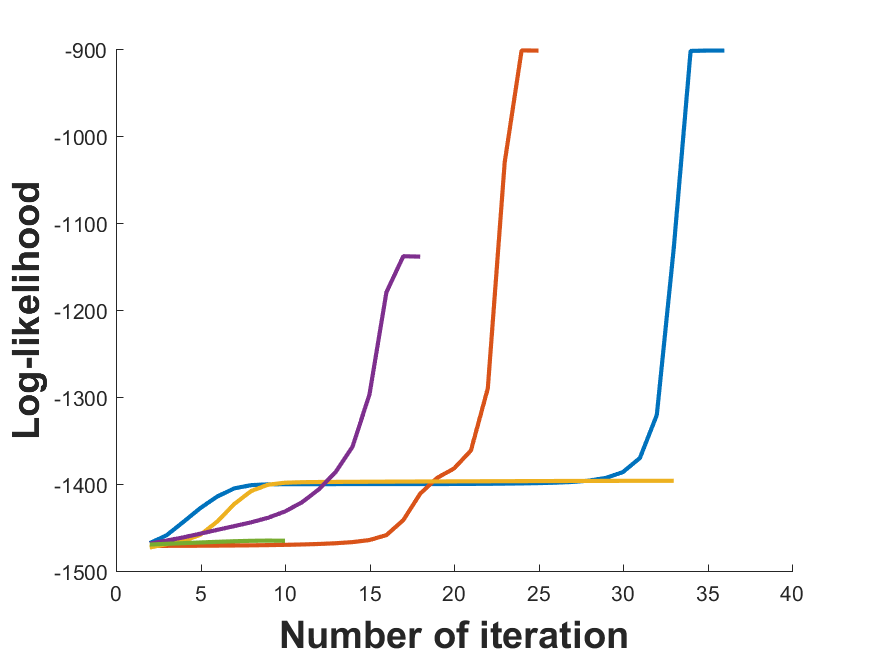
\includegraphics[width=0.75\linewidth]{init_fhmm.png} 
    \caption{Exact} 
  \end{subfigure}%% 
  \begin{subfigure}[b]{0.5\linewidth}
    \centering
    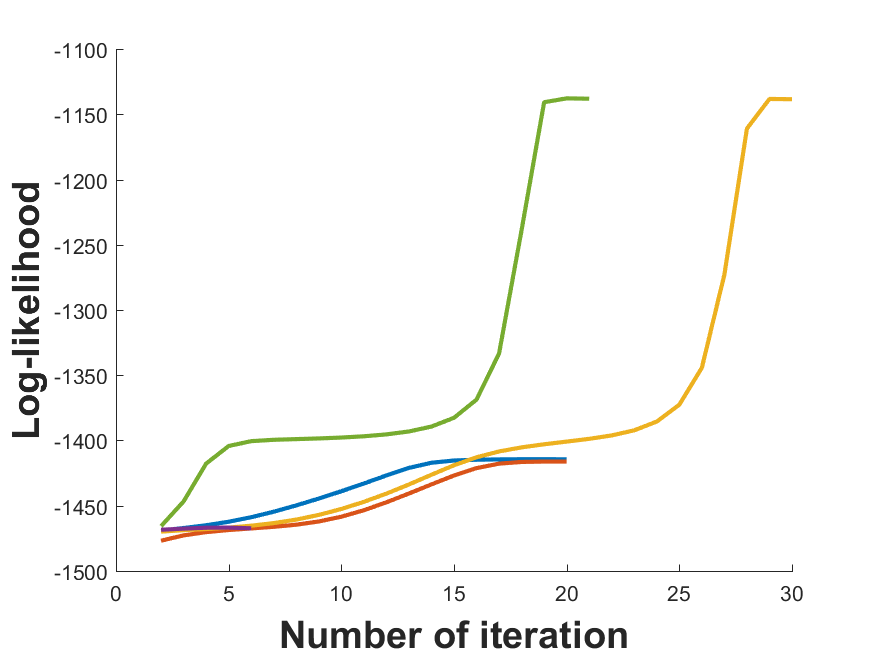
\includegraphics[width=0.75\linewidth]{init_gibbs.png} 
    \caption{Gibbs} 
  \end{subfigure} 
  \begin{subfigure}[b]{0.5\linewidth}
    \centering
    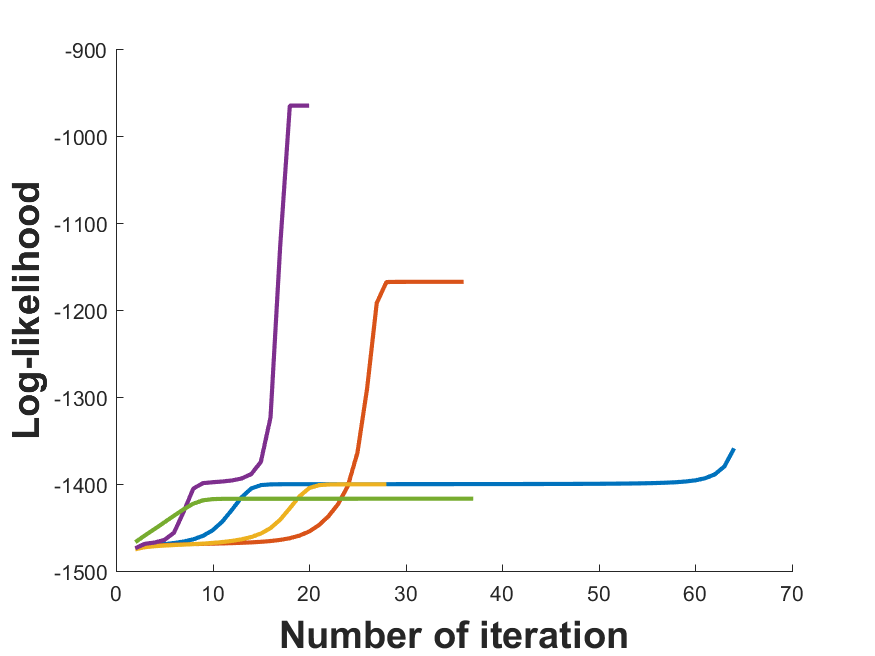
\includegraphics[width=0.75\linewidth]{init_cfva.png} 
    \caption{CFVA} 
  \end{subfigure}%%
  \begin{subfigure}[b]{0.5\linewidth}
    \centering
    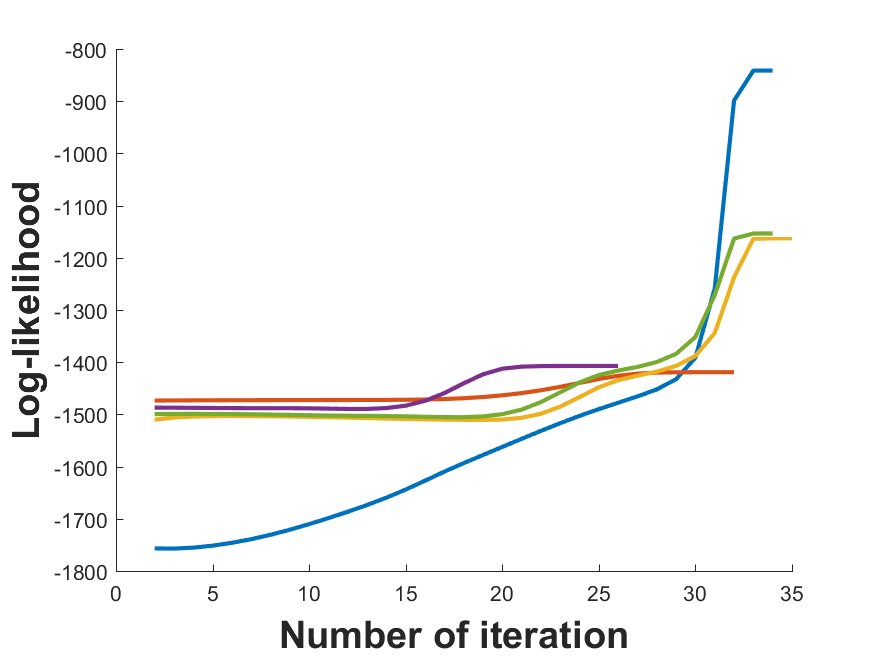
\includegraphics[width=0.75\linewidth]{init_sva.png} 
    \caption{SVA} 
  \end{subfigure} 
  \caption{Learning curves for five runs on the training set for each of the four learning algorithms}
  \label{fig4} 
\end{figure}

HMMs are frequently initialized by a k-means algorithm, but in the case of a factorial HMM, the means of clusters are organized in some patterns, indeed changing one hidden state $S^{(m)}_t$ translates the mean $\mu_t = \sum_{m=1}^M W^{(m)} S_t^{(m)}$, and this translation does not depend of other hidden states. This makes the k-means initialization impossible to use. So we designed another initialization adapted to factorial HMMs and it works as follows :
\begin{verbatim}
For m = 1 to M
    k = kmeans with K centers
    Superpose each cluster k found
    W(m) = k
    P(m) = probabilities of clusters k
endFor
\end{verbatim}
Where the superposition of clusters is just the affectation for each observed points $Y_t = Y_t - k_t$ for $k_t$ the nearest cluster of $Y_t$. Also the affectation of $W$ and $P$ are done hidden state per hidden state.

This reproduces similar patterns of factorial HMMs, and even sometimes found the right centers quite precisely. In practice, the four algorithms founds on average higher local maxima. An example of clusters found by this initialization and the four algorithms is show in figure \ref{fig6}. We see there that the initialization is not very far from the true parameters and that three of the four algorithms gives quite good approximations.

\begin{figure}[h]
	\centering
	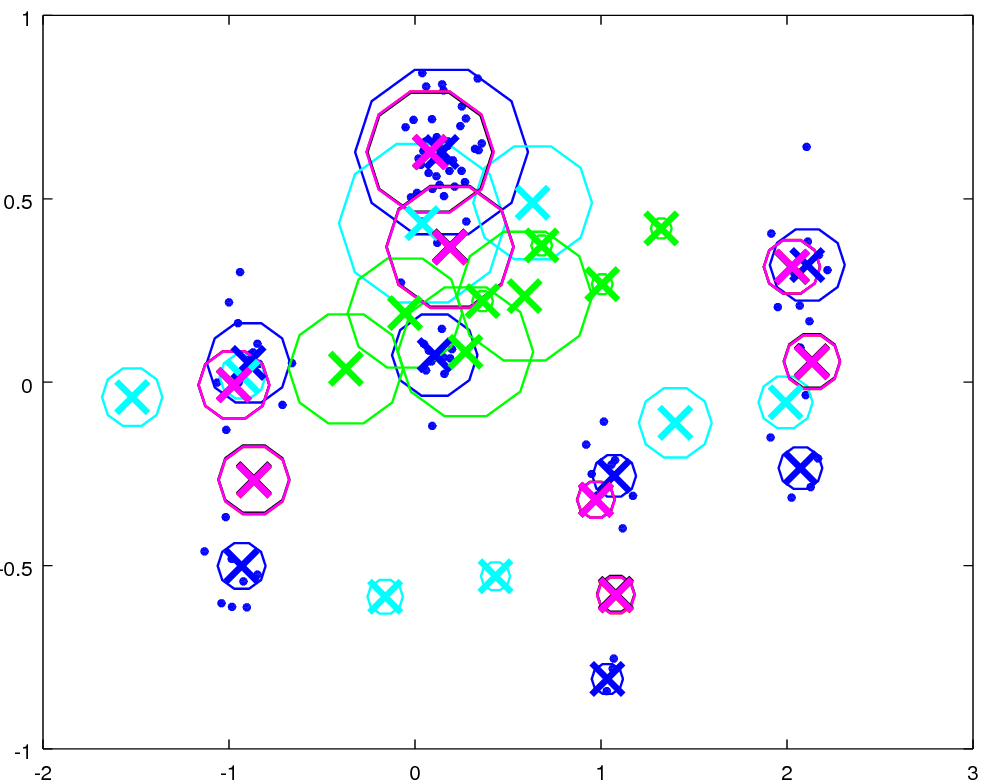
\includegraphics[width=1.0\textwidth]{fig11.png}
	\caption{Centers for synthetic data. Blue dots are the observed points $Y_t$, and we have : Crosses = centers, Circles = probabilities of each center, Blue = True parameters, Light Blue = Our k-means Initialization, Violet = FHMM, CFVA, SVA (they found the same result), Green = Gibbs sampling}
	\label{fig6}
\end{figure}

\subsection{Experiments on real data}

We applied the structural variational approximation on real data. First we choose the dataset "Activity Recognition from Single Chest-Mounted Accelerometer Data Set" from UCI Repository, which records the acceleration of persons during different activities such as walking, going up/down stairs or working at computer. We tried to learn parameters of each of theses activities, and then for a new activity we compute the log-likelihood of each set of parameters, and the set of parameters that gave the biggest log-likelihood would be the recognized activity. In practice the data is not separated in several Gaussians \ref{fig5} so it performs poorly at recognizing activities.

\begin{figure}[h]
	\centering
	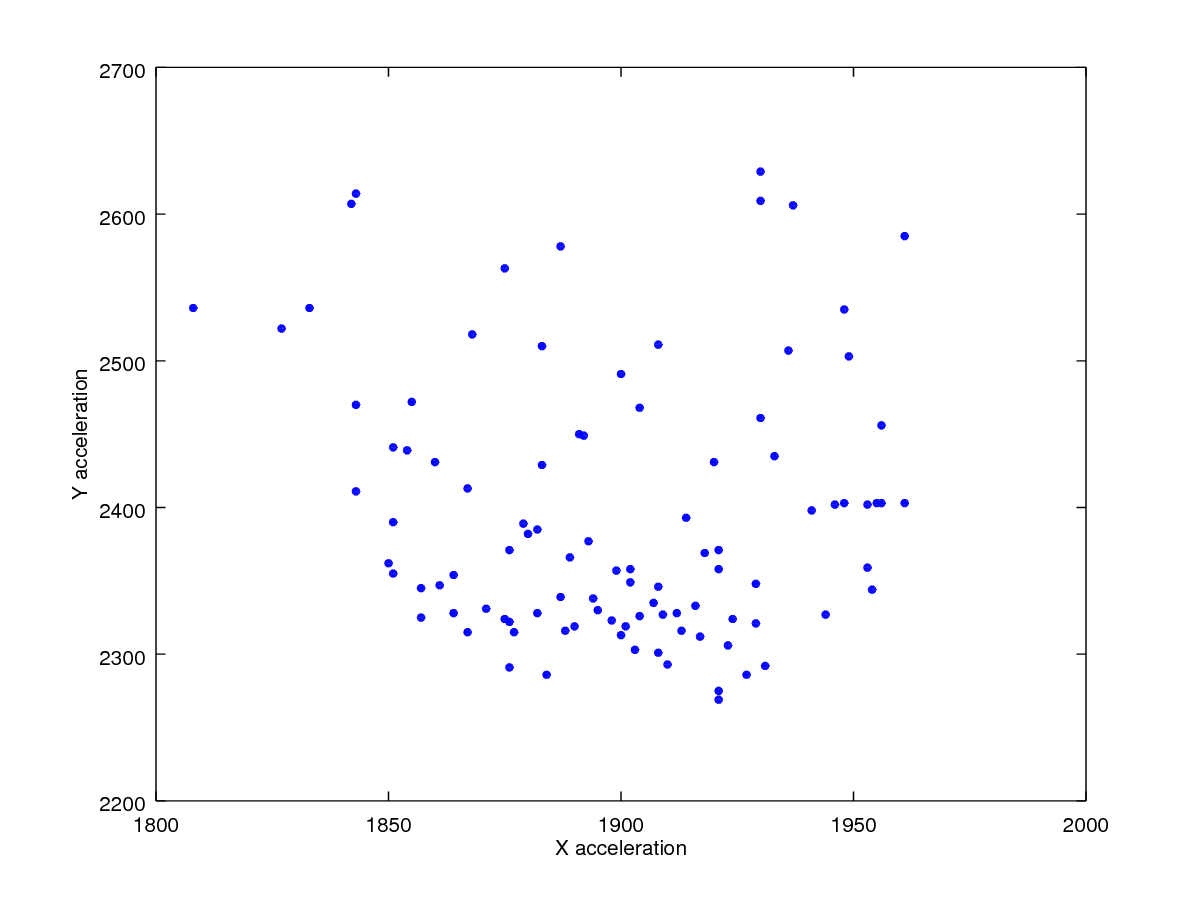
\includegraphics[width=0.5\textwidth]{standing.png}
	\caption{Example of data from Single Chest-Mounted Accelerometer Data Set}
	\label{fig5}
\end{figure}

Then we tried another dataset : CalIt2 Building People Counts Data Set, which counts the number of persons that come in and out of a building. So we expect different cluster such as the beginning of the day when every one comes in and nobody comes out, the night when there is no movement, or the lunch pause when there is many people coming both ways. Unfortunately, here again the dataset does not seem very structured \ref{fig7}.

\begin{figure}[h]
	\begin{minipage}[b]{.49\linewidth}
		\vspace{10pt}
		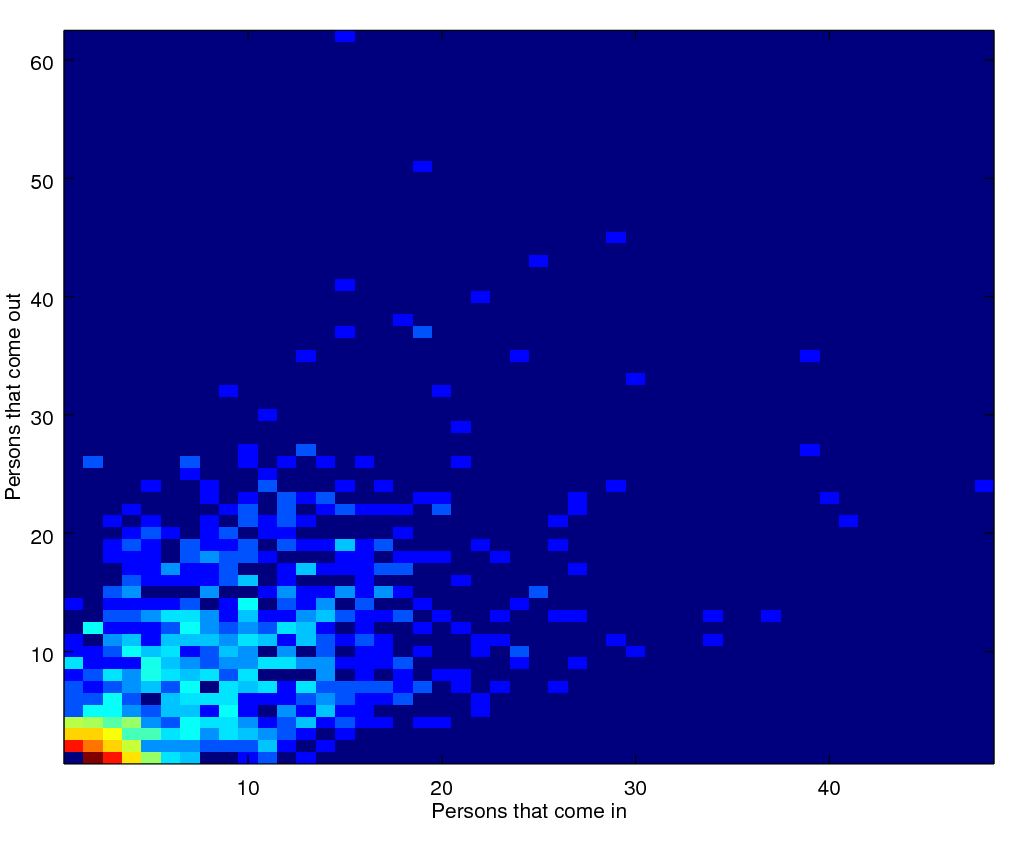
\includegraphics[width=1.0\textwidth]{building.png}
		%  \vspace{1.5cm}
		\begin{center}
			\caption{Example of data from CalIt2 Building People Counts Data Set, red points are frequent points}
			\label{fig7}
		\end{center}\medskip
	\end{minipage}
	\hfill
	\begin{minipage}[b]{0.49\linewidth}
		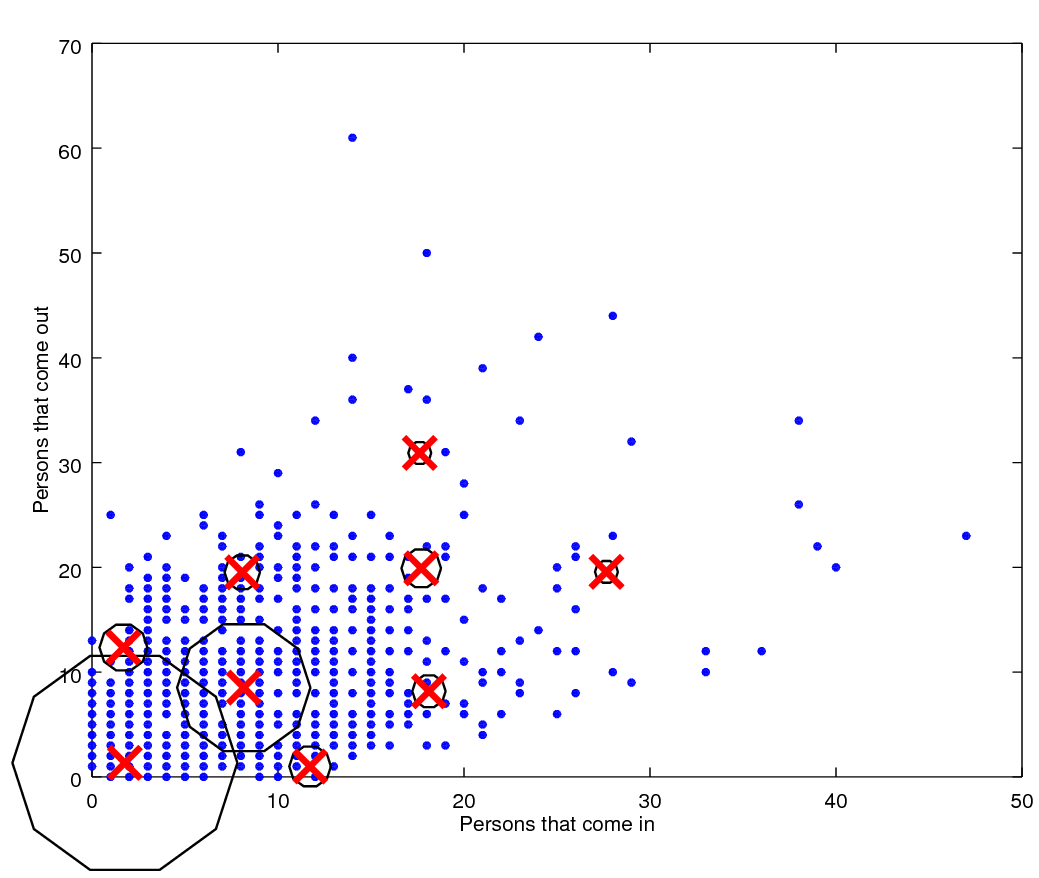
\includegraphics[width=1.0\textwidth]{expe4.png}
		%  \vspace{1.5cm}
		\begin{center}
			\caption{Centers found by structural variational approximation with the parameters $M = 2$ and $K = 3$}
			\label{fig8}
		\end{center}\medskip
	\end{minipage}
\end{figure}

In figure \ref{fig8}, we observe that the algorithm catches the global cluster in the center and the cluster on the bottom-left corner but other clusters are a little useless.

\clearpage
\section{Conclusion}

HMMs are used a lot and the factorial HMMs offers a generalization and a speed up in learning time-series probabilistic models. But in order to be efficient, the data must have regular clusters, organized in some patterns and few dataset have theses patterns. Moreover, the assumption that the covariance matrix is the same for each cluster seems false in many cases.
\newline

Thus, further work should relax the covariance matrix equality for each cluster. It may also be helpful to add some links between each parallel HMM to match more complicated data, without being limited to match patterns, but these links should be added with parsimony as it quickly complicates the model.


\section*{References}

\small

[1] Z. Ghahramani and M. I. Jordan, ``Factorial Hidden Markov Models'', \it{Machine Learning}, vol. 29, pp. 245-273, 1997.

\normalsize

\appendix

\section{The M step}

In our model, the log-likelihood is given by:
\begin{align*}
\ell = &-\frac{1}{2} \sum_{t=1}^T \Bigg[Y_t^\mathsf{T} C^{-1} Y_t - 2 \sum_{m=1}^M Y_t^\mathsf{T} C^{-1} W^{(m)} \langle S_t^{(m)} \rangle + \sum_{m=1}^M \sum_{n=1}^M \Tr\bigg\{ W^{(m)^\mathsf{T}} C^{-1} W^{(m)} \langle S_{t-1}^{(m)} S_{t}^{(m)^\mathsf{T}} \rangle \bigg\} \Bigg] \\
&+ \sum_{m=1}^M \langle S_1^{(m)^\mathsf{T}} \rangle \log \pi^{(m)} + \sum_{t=2}^T \sum_{m=1}^M \Tr\Big\{ \log P^{(m)} \langle S_{t-1}^{(m)} S_{t}^{(m)^\mathsf{T}} \rangle \Big\} - \log Z
\end{align*} 
where Z is a normalization term.

We assume $Y_t$ is a $D \times 1$ vector and we let $S_t$ be the $MK \times 1$ vector obtained by concatenating the $S^{(m)}$ vectors and $W$ be the $D \times MK$ matrix obtained by concatenating the $W^{(m)}$ matrices (of size $D \times K$). Setting the derivatives of $\ell$ with respect to the different parameters to zero, we obtain the following results

\[ W^\textnormal{new} = \Bigg( \sum_{t=1}^T Y_t \langle S_{t}^\mathsf{T} \rangle \Bigg) \Bigg( \sum_{t=1}^T \langle S_{t} S_{t}^\mathsf{T} \rangle \Bigg)^\dagger \qquad \pi^{(m) \ \textnormal{new}} = \langle S_{1}^{(m)}  \rangle\]

\[ P_{i,j}^{(m) \ \textnormal{new}} = \frac{\sum_{t=2}^T \langle S_{t,i}^{(m)} S_{t-1,j}^{(m)}  \rangle}{\sum_{t=2}^T \langle S_{t-1,j}^{(m)}  \rangle} \qquad C^{\textnormal{new}} = \frac{1}{T} \sum_{t=1}^T Y_t Y_t^\mathsf{T} - \frac{1}{T} \sum_{t=1}^T \sum_{m=1}^M W^{(m)} \langle S_t^{(m)} Y_t^\mathsf{T} \rangle \]
where $\dagger$ is the Moore-Penrose pseudo-inverse.

\section{Exact forward-backward algorithm}

Here we describe an exact forward-backward recursion which uses the independence of the Markov chains. Recall that $\phi$ denote the parameters of our model and using the notation $\{ Y_\tau \}_t^r$ to mean the observation sequence $Y_t,\dots,Y_r$, we define:
\begin{align*}
\alpha_t &= P(S_t^{(1)},\dots,S_t^{(M)}, \{Y_\tau \}_1^t | \phi) \\
\alpha_t^{(0)} &= P(S_t^{(1)},\dots,S_t^{(M)}, \{Y_\tau \}_1^{t-1} | \phi) \\
\alpha_t^{(1)} &= P(S_{t-1}^{(1)},\dots,S_t^{(M)}, \{Y_\tau \}_1^{t-1} | \phi) \\
&\vdots \\
\alpha_t^{(M)} &= P(S_{t-1}^{(1)},\dots,S_{t-1}^{(M)}, \{Y_\tau \}_1^{t-1} | \phi)
\end{align*}

Then we obtain the forward recursions:
\[ \alpha_t = P(Y_t | S_t^{(1)},\dots,S_t^{(M)}, \phi) \alpha_t^{(0)} \qquad \alpha_t^{(m-1)} = \sum_{S_{t-1}^{(m)}} P(S_t^{(m)} | S_{t-1}^{(m)}) \alpha_t^{(m)} \]

Similarly for the backward recursions we define:
\begin{align*}
\beta_t &= P(\{Y_\tau \}_{t+1}^T | S_t^{(1)},\dots,S_t^{(M)}, \phi) \\
\beta_{t-1}^{(M)} &= P(\{Y_\tau \}_{t}^T | S_t^{(1)},\dots,S_t^{(M)}, \phi) \\
&\vdots \\ 
\beta_{t-1}^{(1)} &= P(\{Y_\tau \}_{t}^T | S_t^{(1)}, S_{t-1}^{(1)}, \dots,S_{t-1}^{(M)}, \phi) \\
\beta_{t-1}^{(0)} &= \beta_{t-1}
\end{align*}

And obtain:
\[ \beta_{t-1}^{(M)} = P(Y_t | S_t^{(1)},\dots,S_t^{(M)}, \phi) \beta_t \qquad \beta_{t-1}^{(m-1)} = \sum_{S_{t}^{(m)}} P(S_t^{(m)} | S_{t-1}^{(m)}) \beta_{t-1}^{(m)} \]

Then the posterior probability of the state at time t is given by:
\[ \gamma_t = \frac{\alpha_t \beta_t}{\sum_{S_t} \alpha_t \beta_t} \]

Using $\alpha_t$, $\beta_t$ and $\gamma_t$, the quantities required for the M step are given by:
\begin{align*}
\langle S_t^{(m)} \rangle &= \sum_{S_t^{(n)} (n \ne m)} \gamma_t \\
\langle S_t^{(m)} S_t^{(n)^\mathsf{T}} \rangle &= \sum_{S_t^{(n)} (r \ne m,n)} \gamma_t \\
\langle S_{t-1}^{(m)} S_t^{(m)^\mathsf{T}} \rangle &= \frac{\sum_{S_{t-1}^{(n)},S_t^{(r)} (n,r \ne m)} \alpha_{t-1} P(S_t | S_{t-1}) P(Y_t | S_t) \beta_t}{\sum_{S_{t-1},S_t} \alpha_{t-1} P(S_t | S_{t-1}) P(Y_t | S_t) \beta_t}
\end{align*}

\section{Completely factorized variational approximation}

From the definition of the variational distribution, we have:
\begin{align*}
\langle S_t^{(m)} \rangle &= \theta_t^{(m)} \\
\langle S_{t-1}^{(m)} S_t^{(m)^\mathsf{T}} \rangle &= \theta_{t-1}^{(m)} \theta_t^{(m)^\mathsf{T}} \\
\langle S_t^{(m)} S_t^{(n)^\mathsf{T}} \rangle &= \left\{
  \begin{array}{rcr}
    \theta_{t}^{(m)} \theta_t^{(n)^\mathsf{T}} \quad \textnormal{if} \ \ m \ne n \\
    diag\Big\{\theta_t^{(m)}\Big\} \quad \textnormal{if} \ \ m = n \\
  \end{array}
\right.
\end{align*}

The KL divergence can therefore be written as:

\begin{align*}
KL = &\sum_{t=1}^T \sum_{m=1}^M \theta_t^{(m)^\mathsf{T}} \log \theta_t^{(m)} + \frac{1}{2} \sum_{t=1}^T \Bigg[ Y_t^\mathsf{T} C^{-1} Y_t - 2 \sum_{m=1}^M Y_t^\mathsf{T} C^{-1} W^{(m)} \theta_t^{(m)} \\
&+ \sum_{m=1}^M \sum_{n \ne m} \Tr\bigg\{ W^{(m)^\mathsf{T}} C^{-1} W^{(n)} \theta_t^{(n)} \theta_t^{(m)^\mathsf{T}} \bigg\} + \sum_{m=1}^M \Tr\bigg\{ W^{(m)^\mathsf{T}} C^{-1} W^{(m)} diag\Big\{\theta_t^{(m)}\Big\} \bigg\} \Bigg] \\
&+ \sum_{m=1}^M \theta_1^{(m)^\mathsf{T}} \log \pi^{(m)} + \sum_{t=2}^T \sum_{m=1}^M \Tr\bigg\{ \theta_{t-1}^{(m)} \theta_t^{(m)^\mathsf{T}} \log P^{(m)} \bigg\} - \log Z_Q + \log Z
\end{align*}

Setting the derivative with respect to $\theta_t^{(m)}$ to zero, we obtain equation \ref{eq2}.

\section{Structured approximation}

For the structured approximation, the KL divergence is given by:
\begin{align*}
KL = &\sum_{t=1}^T \sum_{m=1}^M \langle S_t^{(m)} \rangle \log h_t^{(m)} + \frac{1}{2} \sum_{t=1}^T \Bigg[ Y_t^\mathsf{T} C^{-1} Y_t - 2 \sum_{m=1}^M Y_t^\mathsf{T} C^{-1} W^{(m)} \langle S_t^{(m)} \rangle \\
&+ \sum_{m=1}^M \sum_{n \ne m} \Tr\bigg\{ W^{(m)^\mathsf{T}} C^{-1} W^{(n)} \langle S_t^{(n)} \rangle \langle S_t^{(m)^\mathsf{T}} \rangle \bigg\} \\
&+ \sum_{m=1}^M \Tr\bigg\{ W^{(m)^\mathsf{T}} C^{-1} W^{(m)} diag\Big\{\langle S_t^{(m)} \rangle\Big\} \bigg\} \Bigg] - \log Z_Q + \log Z
\end{align*}

Taking derivatives with respect to $\log h_t^{(n)}$ and setting it to zero yields equation \ref{eq3}.

\end{document}


